\centering

\begin{minipage}[t]{0.6\textwidth}
\centering
\scalebox{0.57}{
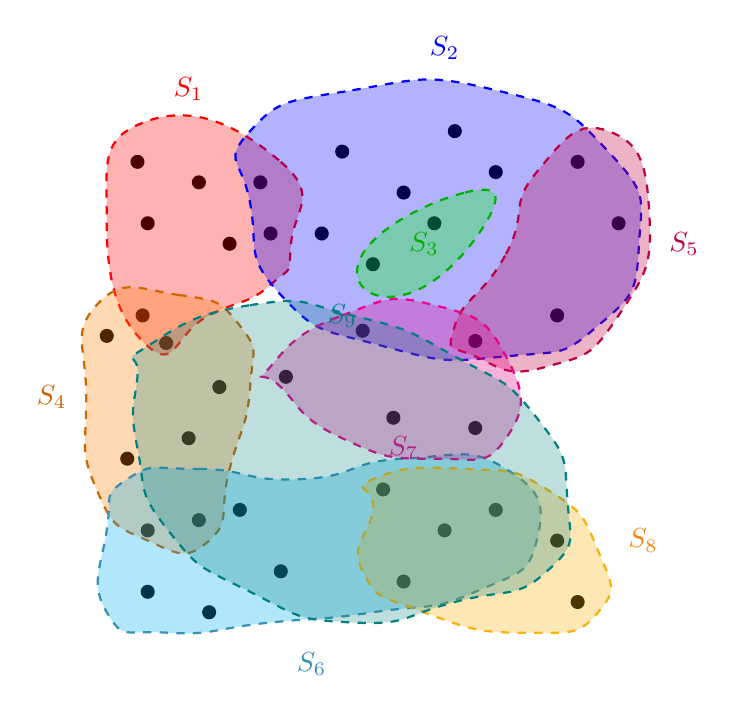
\begin{tikzpicture}[
    scale=1.3,
    node distance=1cm,
    element/.style={circle, draw, thick, fill=black, minimum size=0.15cm, inner sep=0pt},
    arrow/.style={->, thick}
]

% Universe elements - scattered randomly across the plane (35 elements with varied distribution)
\node[element] at (0.4, 3.9) {};
\node[element] at (0.9, 4.3) {};
\node[element] at (1.2, 3.7) {};
\node[element] at (0.35, 3) {};
\node[element] at (1.5, 4.3) {};
\node[element] at (0.3, 4.5) {};
\node[element] at (1.6, 3.8) {};  % SHARED by S1 and S2
\node[element] at (0.58, 2.73) {};  % SHARED by S1 and S4

\node[element] at (2.3, 4.6) {};
\node[element] at (2.9, 4.2) {};
\node[element] at (2.1, 3.8) {};
\node[element] at (3.4, 4.8) {};
\node[element] at (3.8, 4.4) {};
\node[element] at (2.6, 3.5) {};
\node[element] at (3.2, 3.9) {};

\node[element] at (4.6, 4.5) {};
\node[element] at (5, 3.9) {};
\node[element] at (4.4, 3) {};

\node[element] at (0, 2.8) {};
\node[element] at (1.1, 2.3) {};
\node[element] at (0.8, 1.8) {};
\node[element] at (0.2, 1.6) {};

\node[element] at (2.5, 2.85) {};
\node[element] at (3.6, 1.9) {};
\node[element] at (2.8, 2) {};
\node[element] at (3.6, 2.75) {};
\node[element] at (1.75, 2.4) {};

\node[element] at (0.9, 1.0) {};  % SHARED by S4 and S6
\node[element] at (0.4, 0.9) {};
\node[element] at (1.3, 1.1) {};
\node[element] at (0.4, 0.3) {};
\node[element] at (1.7, 0.5) {};
\node[element] at (1.0, 0.1) {};

\node[element] at (2.7, 1.3) {};
\node[element] at (3.3, 0.9) {};
\node[element] at (2.9, 0.4) {};
\node[element] at (3.8, 1.1) {};
\node[element] at (4.4, 0.8) {};
\node[element] at (4.6, 0.2) {};

% Set S1 (red) - includes (0.4,3.9) (0.9,4.3) (1.2,3.7) (0.6,3.2) (1.5,4.1) (0.3,4.5) + SHARED (1.6,4.0) (0.9,2.9)
\draw[thick, dashed, red, fill=red, fill opacity=0.3] 
    plot[smooth cycle, tension=1.0] coordinates {(0.4,4.9) (1.7,4.5) (1.8,3.7) (1.6,3.3) (1.0, 3) (0.4,2.7) (0.0,3.9)};
\node[above] at (0.8,5.0) {\textcolor{red}{$S_1$}};

% Set S2 (blue) - includes (2.3,4.6) (2.9,4.2) (2.1,3.8) (3.4,4.8) (3.8,4.4) (2.6,3.5) (3.2,3.9) (4.3,4.5) (4.7,3.9) (4.1,3.4) + SHARED (1.6,4.0)
\draw[thick, dashed, blue, fill=blue, fill opacity=0.3]
    plot[smooth cycle, tension=1.0] coordinates {(1.4,4.8) (2.4,5.2) (3.8,5.2) (4.9,4.6) (5.2,3.7) (4.8,2.9) (3.9,2.6) (2.7,2.7) (1.7,3.2) (1.4,4.1)};
\node[above] at (3.3,5.4) {\textcolor{blue}{$S_2$}};

% Set S3 (green) - small subset inside S2: (2.6,3.5) (3.2,3.9)
\draw[thick, dashed, green!70!black, fill=green, fill opacity=0.3]
    plot[smooth cycle, tension=1.0] coordinates {(2.5,3.6) (3.5,4.2) (3.7,3.9) (2.9,3.2)};
\node at (3.1,3.7) {\textcolor{green!70!black}{$S_3$}};

% Set S4 (orange) - includes (0.5,2.5) (1.1,2.8) (0.8,2.0) (0.2,1.6) + SHARED (0.9,1.0) (0.9,2.9)
\draw[thick, dashed, orange!80!black, fill=orange, fill opacity=0.3]
    plot[smooth cycle, tension=1.0] coordinates {(-0.1,3.1) (0.7,3.2) (1.3,2.9) (1.4,2.3) (1.2,1.5) (1.0,0.8) (0.4,0.8) (-0.1,1.3) (-0.2,2.2)};
\node[left] at (-0.3,2.2) {\textcolor{orange!80!black}{$S_4$}};

% Set S5 (purple) - right side elongated: (3.6,2.6) overlaps with S2 for (4.3,4.5) (4.7,3.9) (4.1,3.4)
\draw[thick, dashed, purple, fill=purple, fill opacity=0.3]
    plot[smooth cycle, tension=1.0] coordinates {(3.4,2.9) (3.9,3.6) (4.2,4.4) (4.9,4.8) (5.3,4.0) (5.0,3.0) (4.3,2.5) (3.6,2.6)};
\node[right] at (5.4,3.7) {\textcolor{purple}{$S_5$}};

% Set S6 (cyan) - includes (0.9,1.0) (0.7,0.8) (1.3,1.1) (0.4,0.3) (1.7,0.5) (1.0,0.1) (2.7,1.3) (3.3,0.9) (2.9,0.4) (3.8,1.1)
\draw[thick, dashed, cyan!70!black, fill=cyan, fill opacity=0.3]
    plot[smooth cycle, tension=1.0] coordinates {(0.2,1.4) (0.9,1.5) (1.9,1.4) (2.9,1.6) (3.9,1.5) (4.2,0.8) (3.6,0.3) (2.6,0.1) (1.6,0.0) (0.6,-0.1) (0.0,0.1) (0.0,0.9)};
\node[below] at (2.0,-0.2) {\textcolor{cyan!70!black}{$S_6$}};

% Set S7 (magenta) - includes (2.5,2.9) (3.1,2.4) (2.8,1.9) (1.9,2.2)
\draw[thick, dashed, magenta, fill=magenta, fill opacity=0.3]
    plot[smooth cycle, tension=1.0] coordinates {(1.6,2.5) (2.3,3.0) (3.2,3.1) (3.9,2.6) (3.9,1.8) (3.2,1.6) (2.3,1.8) (1.7,2.3)};
\node[above] at (2.9,1.5) {\textcolor{magenta}{$S_7$}};

% Set S8 (yellow!70!red) - includes (3.8,1.1) (4.4,0.6) (3.3,0.9) (2.9,0.4)
\draw[thick, dashed, yellow!70!red, fill=yellow!70!red, fill opacity=0.3]
    plot[smooth cycle, tension=1.0] coordinates {(2.6,1.4) (3.5,1.5) (4.3,1.3) (4.8,0.7) (4.8,0.1) (4.1,-0.1) (3.1,0.1) (2.5,0.5) (2.6,1.1)};
\node[right] at (5.0,0.8) {\textcolor{yellow!50!red}{$S_8$}};

% Set S9 (teal) - large blob filling gaps: overlaps with others to ensure complete coverage
\draw[thick, dashed, teal, fill=teal, fill opacity=0.25]
    plot[smooth cycle, tension=1.0] coordinates {(0.4,2.7) (1.4,3.1) (2.4,3.0) (3.4,2.6) (4.2,2.0) (4.5,1.2) (4.3,0.5) (3.4,0.2) (2.4,0.0) (1.4,0.3) (0.6,0.9) (0.3,1.7) (0.3,2.4)};
\node[below] at (2.3,3.2) {\textcolor{teal}{$S_9$}};

\end{tikzpicture}
}
\normalsize
\caption*{(a) Universe and sets}
\end{minipage}
\hfill
\begin{minipage}[t]{0.35\textwidth}
\centering
\scalebox{0.57}{
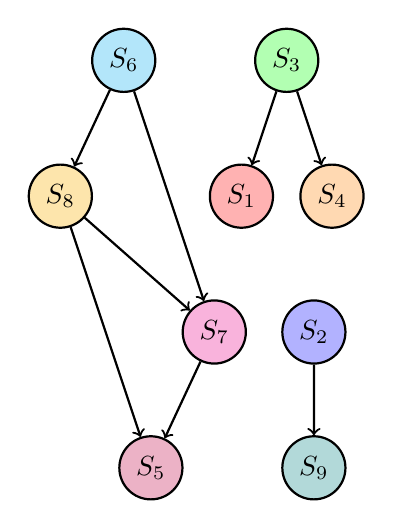
\begin{tikzpicture}[
    scale=1.15,
    node distance=1cm,
    set/.style={circle, draw, thick, minimum size=0.65cm},
    arrow/.style={->, thick}
]

% Precedence DAG with specified precedence constraints

% Component with S6 (left, wider)
\node[set, fill=cyan!30] (s6) at (0,0) {$S_6$};
\node[set, fill=yellow!70!red!30] (s8) at (-0.7,-1.5) {$S_8$};
\node[set, fill=magenta!30] (s7) at (1,-3) {$S_7$};
\node[set, fill=purple!30] (s5) at (0.3,-4.5) {$S_5$};

% Component with S3 (right top)
\node[set, fill=green!30] (s3) at (1.8,0) {$S_3$};
\node[set, fill=red!30] (s1) at (1.3,-1.5) {$S_1$};
\node[set, fill=orange!30] (s4) at (2.3,-1.5) {$S_4$};

% Component with S2 (right bottom)
\node[set, fill=blue!30] (s2) at (2.1,-3) {$S_2$};
\node[set, fill=teal!30] (s9) at (2.1,-4.5) {$S_9$};

% Precedence constraints (all arrows go down)
\draw[arrow] (s3) -- (s1);
\draw[arrow] (s3) -- (s4);
\draw[arrow] (s6) -- (s7);
\draw[arrow] (s6) -- (s8);
\draw[arrow] (s8) -- (s7);
\draw[arrow] (s8) -- (s5);
\draw[arrow] (s7) -- (s5);
\draw[arrow] (s2) -- (s9);

\end{tikzpicture}
}
\normalsize
\caption*{(b) Precedence}
\end{minipage}

\vspace{0.5cm}

\begin{minipage}[t]{\textwidth}
\centering
\scalebox{0.765}{
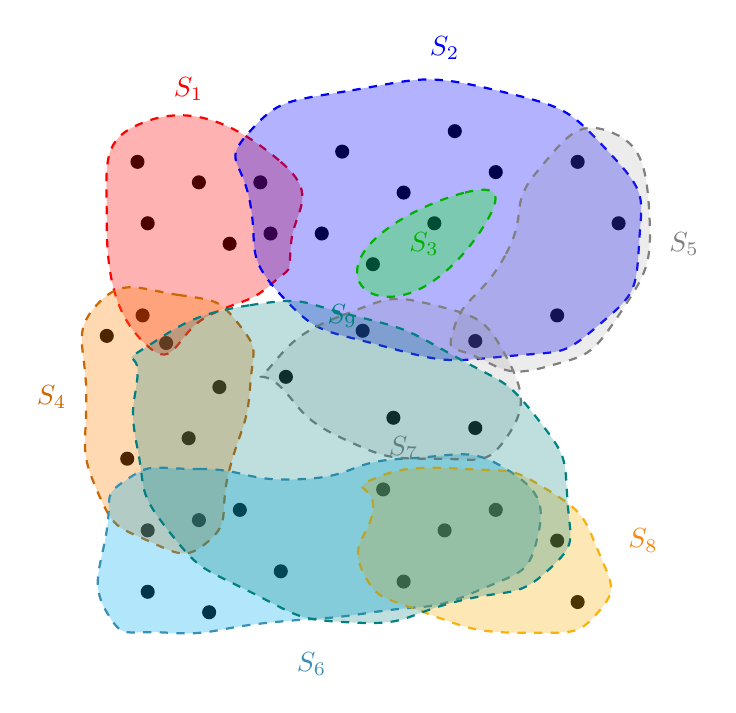
\begin{tikzpicture}[
    scale=1.3,
    node distance=1cm,
    element/.style={circle, draw, thick, fill=black, minimum size=0.15cm, inner sep=0pt},
    arrow/.style={->, thick}
]

% Universe elements - scattered randomly across the plane (35 elements with varied distribution)
\node[element] at (0.4, 3.9) {};
\node[element] at (0.9, 4.3) {};
\node[element] at (1.2, 3.7) {};
\node[element] at (0.35, 3) {};
\node[element] at (1.5, 4.3) {};
\node[element] at (0.3, 4.5) {};
\node[element] at (1.6, 3.8) {};  % SHARED by S1 and S2
\node[element] at (0.58, 2.73) {};  % SHARED by S1 and S4

\node[element] at (2.3, 4.6) {};
\node[element] at (2.9, 4.2) {};
\node[element] at (2.1, 3.8) {};
\node[element] at (3.4, 4.8) {};
\node[element] at (3.8, 4.4) {};
\node[element] at (2.6, 3.5) {};
\node[element] at (3.2, 3.9) {};

\node[element] at (4.6, 4.5) {};
\node[element] at (5, 3.9) {};
\node[element] at (4.4, 3) {};

\node[element] at (0, 2.8) {};
\node[element] at (1.1, 2.3) {};
\node[element] at (0.8, 1.8) {};
\node[element] at (0.2, 1.6) {};

\node[element] at (2.5, 2.85) {};
\node[element] at (3.6, 1.9) {};
\node[element] at (2.8, 2) {};
\node[element] at (3.6, 2.75) {};
\node[element] at (1.75, 2.4) {};

\node[element] at (0.9, 1.0) {};  % SHARED by S4 and S6
\node[element] at (0.4, 0.9) {};
\node[element] at (1.3, 1.1) {};
\node[element] at (0.4, 0.3) {};
\node[element] at (1.7, 0.5) {};
\node[element] at (1.0, 0.1) {};

\node[element] at (2.7, 1.3) {};
\node[element] at (3.3, 0.9) {};
\node[element] at (2.9, 0.4) {};
\node[element] at (3.8, 1.1) {};
\node[element] at (4.4, 0.8) {};
\node[element] at (4.6, 0.2) {};

% Set S1 (red) - SELECTED
\draw[thick, dashed, red, fill=red, fill opacity=0.3] 
    plot[smooth cycle, tension=1.0] coordinates {(0.4,4.9) (1.7,4.5) (1.8,3.7) (1.6,3.3) (1.0, 3) (0.4,2.7) (0.0,3.9)};
\node[above] at (0.8,5.0) {\textcolor{red}{\textbf{$S_1$}}};

% Set S2 (blue) - SELECTED
\draw[thick, dashed, blue, fill=blue, fill opacity=0.3]
    plot[smooth cycle, tension=1.0] coordinates {(1.4,4.8) (2.4,5.2) (3.8,5.2) (4.9,4.6) (5.2,3.7) (4.8,2.9) (3.9,2.6) (2.7,2.7) (1.7,3.2) (1.4,4.1)};
\node[above] at (3.3,5.4) {\textcolor{blue}{\textbf{$S_2$}}};

% Set S3 (green) - SELECTED
\draw[thick, dashed, green!70!black, fill=green, fill opacity=0.3]
    plot[smooth cycle, tension=1.0] coordinates {(2.5,3.6) (3.5,4.2) (3.7,3.9) (2.9,3.2)};
\node at (3.1,3.7) {\textcolor{green!70!black}{\textbf{$S_3$}}};

% Set S4 (orange) - SELECTED
\draw[thick, dashed, orange!80!black, fill=orange, fill opacity=0.3]
    plot[smooth cycle, tension=1.0] coordinates {(-0.1,3.1) (0.7,3.2) (1.3,2.9) (1.4,2.3) (1.2,1.5) (1.0,0.8) (0.4,0.8) (-0.1,1.3) (-0.2,2.2)};
\node[left] at (-0.3,2.2) {\textcolor{orange!80!black}{\textbf{$S_4$}}};

% Set S5 (purple) - NOT SELECTED (grayed out)
\draw[thick, dashed, gray, fill=gray, fill opacity=0.15]
    plot[smooth cycle, tension=1.0] coordinates {(3.4,2.9) (3.9,3.6) (4.2,4.4) (4.9,4.8) (5.3,4.0) (5.0,3.0) (4.3,2.5) (3.6,2.6)};
\node[right] at (5.4,3.7) {\textcolor{gray}{$S_5$}};

% Set S6 (cyan) - SELECTED
\draw[thick, dashed, cyan!70!black, fill=cyan, fill opacity=0.3]
    plot[smooth cycle, tension=1.0] coordinates {(0.2,1.4) (0.9,1.5) (1.9,1.4) (2.9,1.6) (3.9,1.5) (4.2,0.8) (3.6,0.3) (2.6,0.1) (1.6,0.0) (0.6,-0.1) (0.0,0.1) (0.0,0.9)};
\node[below] at (2.0,-0.2) {\textcolor{cyan!70!black}{\textbf{$S_6$}}};

% Set S7 (magenta) - NOT SELECTED (grayed out)
\draw[thick, dashed, gray, fill=gray, fill opacity=0.15]
    plot[smooth cycle, tension=1.0] coordinates {(1.6,2.5) (2.3,3.0) (3.2,3.1) (3.9,2.6) (3.9,1.8) (3.2,1.6) (2.3,1.8) (1.7,2.3)};
\node[above] at (2.9,1.5) {\textcolor{gray}{$S_7$}};

% Set S8 (yellow!70!red) - SELECTED
\draw[thick, dashed, yellow!70!red, fill=yellow!70!red, fill opacity=0.3]
    plot[smooth cycle, tension=1.0] coordinates {(2.6,1.4) (3.5,1.5) (4.3,1.3) (4.8,0.7) (4.8,0.1) (4.1,-0.1) (3.1,0.1) (2.5,0.5) (2.6,1.1)};
\node[right] at (5.0,0.8) {\textcolor{yellow!50!red}{\textbf{$S_8$}}};

% Set S9 (teal) - SELECTED
\draw[thick, dashed, teal, fill=teal, fill opacity=0.25]
    plot[smooth cycle, tension=1.0] coordinates {(0.4,2.7) (1.4,3.1) (2.4,3.0) (3.4,2.6) (4.2,2.0) (4.5,1.2) (4.3,0.5) (3.4,0.2) (2.4,0.0) (1.4,0.3) (0.6,0.9) (0.3,1.7) (0.3,2.4)};
\node[below] at (2.3,3.2) {\textcolor{teal}{\textbf{$S_9$}}};

\end{tikzpicture}
}
\normalsize
\caption*{(c) Solution: $\{S_1, S_2, S_6, S_8, S_9\}$ (in color)}
\end{minipage}

